% !TeX spellcheck = cs_CZ
\begin{example}\label{TEO:exam014}
  Celková plocha \(S\) na obr. \ref{es:fig_patocka_mag_tok_exp9} leží v rovině \(x-y\) a je 
  sestavena z devíti „diferenciálních“ plošek o velikosti \(dS = \SI{1}{\cm} \cdot \SI{1}{\cm} = 
  \SI{1}{\cm^2}\). Čísla i směry šipek na hranách čtverečků byly zvoleny zcela nahodile. 
  Reprezentují složky \(E_x\), \(E_y\) lokálních intenzit nehomogenního elektrického pole. 
  Intenzity jsou měřeny ve \si{V/\cm}, Uvnitř čtverečků jsou zvoleny směry oběhu. Všechny směry 
  musí být shodné. V souladu s těmito směry je uvnitř každého čtverečku uvedena velikost 
  \(z\)-složky \(\rot{E}_x\) rotace v jednotkách \si{V/\cm^2}, vypočítaná podle rovnice 
  (\ref{ES:eq_zakl_elm34}). Rovnici znovu napíšeme, abychom na ni demonstrovali výpočet 
  \(z\)-složky rotace:
  \begin{equation*}
    (\rot{E})_z   = \left(\pder{E_y}{x} - \pder{E_x}{y}\right)                  
                  = \frac{du_z}{dS_z}
                  = \frac{du_a + du_b + du_c + du_d}{dS_z}.
  \end{equation*}
  V našem konkrétním případě mají všechny čtverečky délku hrany \SI{1}{\cm}, tak lze psát:
  \begin{align*}
    (\rot{E})_z &= \left(\pder{E_y}{x} - \pder{E_x}{y}\right)
                 = \frac{du_z}{dS_z}                                          \\
                &= \frac{E_a\cdot\SI{1}{\cm} + E_b\cdot\SI{1}{\cm} + 
                    E_c\cdot\SI{1}{\cm} + E_d\cdot\SI{1}{\cm}}{dS_z}.
  \end{align*}
  Například pro prostřední čtvereček vychází:
  \begin{align*}
    (\rot{E})_z 
      &= \frac{\SI{3}{V/\cm}\cdot\SI{1}{\cm} + \SI{2}{V/\cm}\cdot\SI{1}{\cm}}{dS_z}  \\
      &- \frac{\SI{1}{V/\cm}\cdot\SI{1}{\cm} - \SI{2}{V/\cm}\cdot\SI{1}{\cm}}{dS_z}   \\
      &= + \SI{2}{V/\cm}.
  \end{align*}
  
   {\centering
    \captionsetup{type=figure}
    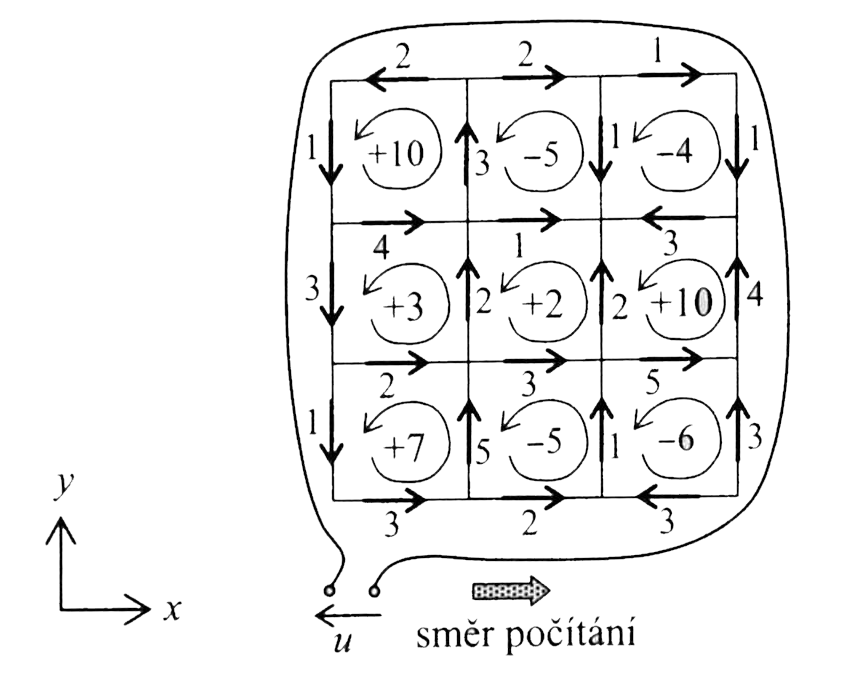
\includegraphics[width=0.7\linewidth]{patocka_mag_tok_exp9.png}
    \captionof{figure}{Konkrétní číselný příklad pro demonstraci Stokesovy věty.}
    \label{es:fig_patocka_mag_tok_exp9}
  \par}
  
  Podle \textbf{Stokesovy věty} lze celkové napětí \(u\) po obvodu velkého čtverce určit dvěma 
  způsoby. První způsob - podle rovnice (\ref{ES:eq_zakl_elm26}):
  \begin{align*}
    u &= \int_l\vec{E}d\vec{l} = \sum\limits_{i=1}^{12}E_i\cdot\SI{1}{\cm}     \\
      &= +3 +2 +3 +3 - 1 - 1 -2 + 2 + 1 + 3 + 1 = + \SI{12}{V}.
  \end{align*}
  Druhý způsob - podle rovnice (\ref{ES:eq_zakl_elm36}):
  \begin{align*}
    u &= \int_S\rot{E} \cdot d\vec{S} 
       = \sum\limits_{j=1}^{9}\left(\rot{E}_z,j\cdot\SI{1}{\cm^2}\right).      \\
      &= + 10 - 5 - 4 + 3 + 2 + 10 + 7 - 5 - 6 = + \SI{12}{V}. 
  \end{align*}
  Oba způsoby dávají opravdu stejný výsledek. Je to geometricky snadno pochopitelné. Všimněme 
  si, že hrany malých čtverečků lze třídit na \emph{vnitřní} (nejsou součástí obvodové křivky) a na 
  \emph{vnější} (jsou součástí obvodové křivky). Kterákoli vnitřní hrana tvoří hranici mezi dvěma 
  sousedními čtverečky. Napětí této hrany přispívá do jednoho čtverečku v kladném smyslu, do 
  sousedního čtverečku v záporném smyslu. Při celkové sumaci počítané druhým způsobem se tedy 
  účinky všech vnitřních hran navzájem zcela zruší a ve výsledku se uplatní napětí pouze vnějších 
  hran — což je totéž, jako bychom počítali prvním způsobem. Poznamenejme, že podobně můžeme na 
  obr. \ref{es:fig_patocka_mag_tok_exp9} spočítat napětí na obvodu libovolné jinak zvolené plochy, 
  např. na obvodu „dolních šesti čtverečků“, na obvodu \emph{„písmene L“} atd. Celý příklad se dá 
  současně chápat jako další částečný návod pro numerické řešení pole metodou konečných prvků.
\end{example}

